\documentclass[a6paper]{article}
\usepackage{polyglossia}
\usepackage[margin=10mm]{geometry}
\usepackage{graphicx}
\setdefaultlanguage{marathi}
\setotherlanguages{english, sanskrit}
%\setmainfont[Mapping=velthuis-sanskrit,Script=Devanagari,Language=Sanskrit]{Shobhika}
\newfontfamily\englishfont{Gentium Book Basic}
\newfontfamily\devanagarifont{Noto Serif Devanagari}
\newfontfamily\marathifont[Mapping=velthuis-sanskrit,Script=Devanagari,Language=Marathi]{Noto Serif Devanagari}
\newfontfamily\sanskritfont[Mapping=velthuis-sanskrit,Script=Devanagari,Language=Sanskrit]{Noto Serif Devanagari}
% make sure ~ as non-breaking space doesn't interfere with velthuis-sanskrit mapping
\edef~{\string~}
\pagenumbering{gobble}
\setlength{\parindent}{0pt}% Remove paragraph indent
\usepackage[skip=\medskipamount]{parskip}
\usepackage{xcolor}
\usepackage{hyperref}
\renewcommand\UrlFont{\ttfamilylatin}
\newcommand \eng[1]{
    \textenglish{#1}
}
% hyphenation https://tex.stackexchange.com/a/177179/64425
\tolerance=1
\emergencystretch=\maxdimen
\hyphenpenalty=10000
\hbadness=10000

\hypersetup{
    colorlinks=true,
    linkcolor=blue,
    filecolor=magenta,
    citecolor=blue,
    urlcolor=purple,
}

\begin{document}

\begin{center}
    {\Large ki"sora!}
\end{center}

rasikaho, namaskaara.

mha.tala.m tara haa (tumacyaa phon cyaa skriin saa.thii .taaiip-se.t kelelaa) lekha itara lekhaa.msaarakhaa `baraaya' asaa jujabii "seraa basuuna tumacyaa d.r.s.tiiaa.da hoiilahii. pa.na kadaacita tumhaalaa kaahiitarii karaayalaa bhaaga paa.dela. prabhaavii likhaa.na ku.thala.m -- tara je kaahii karaayalaa laavata.m te -- asa.m maajha.m mata aahe. tumhii ase k.rtii"siila vaacaka asaala tara saraLa yaa lekhaacaa "seva.ta gaa.thaa aa.ni tithe sucavalelii k.rtii k.rpayaa karaa; haa lekha kaara.nii laagalyaaca.m samaadhaana malaa miLela. te kaama tumhii yaaaadhiica kela.m asela tara uttama -- tumace khuupa aabhaara.

a"sii aagrahii bhuumikaa dhara.nyaamaagaca.m kaara.na asa.m kii te kaama kelyaane malaa ati"saya aana.mda jhaalaa aahe aa.ni tumhaalaahii hoiila. kaliyugaatahii kaahii nitaa.mtasu.mdara go.s.tii gha.dataata yaavara vi"svaasa basela!

maraa.thii (aa.ni itarahii) madhyamamaargii, madhyamavayiina, madhyamavargiiya (mha.naje maajhyaasaarakhyaa) lokaa.mca.m sadhyaaca.m aava.data.m pracaara, prasaara, aa.ni abhivyaktii saadhana jara ku.thala.m asela tara te व्हॉ.tसॅp!  yaa maadhyamaace  kaahii to.te asale tarii tyaata ga.mmata pa.na khuupa aahe -- tho.dii sahana"siilataa, svapraj~nevara vi"svaasa, aa.ni samaajamanaavi.sayii utsukataa asela tara. asmitaa soma.na tara tyaalaa `` व्हॉ.tसॅp vidyaapii.tha '' mha.nate. 

nukatiica  व्हॉ.tसॅp vara  eka kavitaa aalii:


    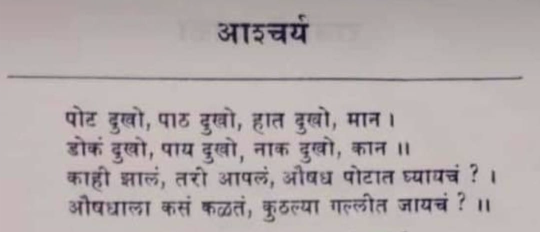
\includegraphics[width=0.7\linewidth]{kishor-p1.png}

aa.ni barobara eka pra"sna -- ``hyaa kavitece kavii ki.mvaa kavayitrii ko.na?''

kavitaa paahataak.sa.nii malaa eka aa.thavala.m -- gharii diipaane malaa hii kavitaa anekadaa mha.nuuna daakhavalii aahe. ekhaadiicii acaa.ta smara.na"saktii aa.ni ticaa itaraa.mvara, vi"se.sata.h maajhyaasaarakhii saamaanya smara.na"saktii asa.naar+yaa.mvara, kasaa pari.naama hoto yaavara punhaa kadhiitarii boluu. 

tine lageca saa.mgitala.m kii kaviteca.m naava `aa"scarya' naahii, tara `au.sadha', aa.ni kavayitrii vijayaa jahaagiiradaara! lahaanapa.nii gharii ye.naar+yaa `ki"sora' madhye aalelii hii kavitaa tine kadhiica paa.tha karuuna .taakalii hotii.

aapalyaa `kaavya-"saastra-vinodaa' cyaa aava.dii-niva.dii.mcaa pratyekaalaaca eka saartha abhimaana asato. malaahii tasaa aahe. maajhyaa cokha.mdaLapa.naavara `ki"sora' caa eka ad.r"sya prabhaava aahe. uttama baa.mdha.nii, suvaacya .ta.mka (\eng{fonts}), caa.mgalyaa pratiica.m prupha-rii.di.mg kelelii bar+yaapaikii chapaaii, thoraamo.thyaa.mnii samarasuuna lihilele vaacaniiya lekha, marmaba.mdhaatalyaa .thevii.msaarakhyaa tarala aa.ni halakyaa-phulakyaa kavitaa, buddhiilaa caalanaa asalelii ko.dii, utka.m.thaavardhaka sadara.m, yathaartha bhaa.saa.mtara.m, ithe-tithe vikhuralele vinodii cu.take, bhuraLa paa.datiila a"sii citra.m, susahya pramaa.naata asalelyaa jaahiraatii, aa.ni yaa sagaLyaa.mvara mulaayama saayiisaarakhaa pasara.naaraa eka mohaka maraa.thamoLaa saadhepa.naa -- a"saa a.mtarbaahya surekha ki"sora maasikaacyaa a.mkaacii aa.thava.na jhaalii kii mana aajahii harakhata.m. ekaaca veLii vaya var.se 8 cyaa pu.dhalyaa kitiihii vayaacyaa maraa.thii vyaktiica.m manora.mjana kara.nyaaca.m saamarthya ki"sora madhye sahajapa.ne saamaavalela.m hota.m, aahe! 

\eng{Robert Heinlein} cyaa mate bhuutakaaLaata ramamaa.na ho.na.m he manaane v.rddhaavastheka.de jhukata caalalyaaca.m cinha aahe. tasa.m te asela tara aso baapa.da.m, pa.na a"sii `gataasiinataa'\footnote{\eng{nostalgia} caa nira.mjanane kelelaa bhaavaanuvaada} sukhaavuuna jaata.m he maatra khara.m!

`ki"sora' cyaa aa.thava.nii.mnii bhaaraavalelaa mii sahaja \eng{Internet} ka.de vaLalo. guugal ne daakhavala.m kii bar+yaaca lokaa.mnaa hyaa go.da baalakavitecyaa ugamaasa.mba.mdhii pra"sna aaheta. malaa vaa.tala.m kii diipaacyaa aaiiva.dilaa.mka.de pahilelaa 1971-1991 madhalyaa sagaLyaa ki"sora-a.mkaa.mca.m baaii.m.di.mg kelelaa sa.mca miLaalaa tara kaaya bahaara yeiila! mii a"saa vicaaraa.mta hoto aa.ni kaaya aa"scarya! malaa \href{https://kishor.balbharati.in/Archives/Index.aspx}{ki"sora-sa.mgraha} yaa sa.mketasthaLaacaa sugaavaa laagalaa. ithe aajavara prakaa"sita jhaalele sagaLe ki"sora maasikaace .diji.tal svaruupaatiila a.mka mophata upalabdha aaheta aa.ni eva.dha.mca naahii tara te tumhaalaa tumacyaa \eng{computer} ki.mvaa phon vara pho.to saarakhe jatanahii karuuna .thevataa ye.nyaacii soya aahe! he malaa ajuunahii khara.m vaa.tata naahii. 

sagaLe a.mka citra-ruupaata (ak.sara-ruupaata navhe) asalyaamuLe ajuunahii ekhaadaa majakuura "sodhaayacii soya mha.naavii titakii sukara jhaalelii naahii. tyaamuLe mii pratyeka a.mka caaLuuna paahilaa aa.ni sarate"seva.tii epril 1979 cyaa a.mkaata malaa sau. vijayaa jahaagiiradaaraa.mnii lihilelii `au.sadha' hii kavitaa saapa.dalii -- aarkimi.dij laa tara.mga.naar+yaa go.s.tii.mce gamaka saapa.dalyaavara jhaalaa asaavaa tasaaca kadaacita aana.mda malaa jhaalaa! aataa maajhyaaka.de puraavaa pa.na hotaa:

    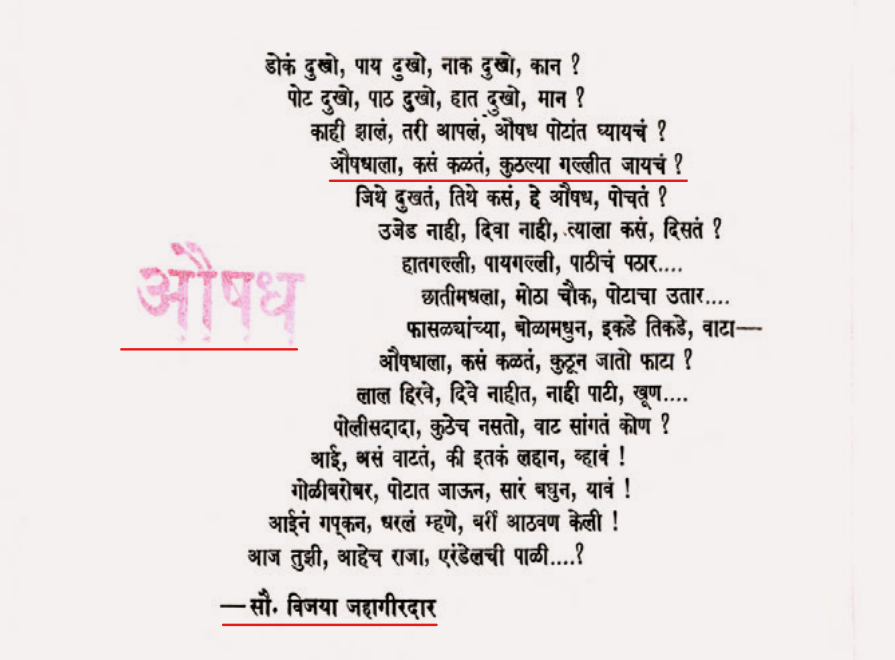
\includegraphics[width=0.8\linewidth]{kishor-p2.png}

kitii vaajavii aahe yaa cho.tyaa"syaa kavitetala.m he niriik.sa.na! aaja re.nuu.mmadhalyaa aakar.sa.naavara sa.m"sodhana karuuna ekhaadyaa ba.dyaa au.sadhaa.mcyaa prathitaya"sa ka.mpaniita kaama kara.naar+yaa \eng{chemist} ki.mvaa \eng {drug-designer} laa yaa kavitene haa bhoLaa pra"sna vicaaruuna janma dilaa nasela ka"saavaruuna?

asa.m he ki"sora maasika. aajahii kaaryarata aahe. prakaa"sita hota aahe! aa.ni vaar.sika varga.nii kitii, tara \textbf{80 ruupaye maatra}! hoya, 2022 madhye yaa apratima maasikaacii vaar.sika varga.nii aahe 80 ruupaye! tyaata tumhaalaa miLate varga.niidaara asalyaacii gvaahii, tumaca.m varga.niidaaraaca.m \eng{home page} (tyaa.mcyaa \eng{portal} vara) aa.ni 12 a.mka var.saalaa gharapoca. vi"svaasa basatoya tumacaa? naahii naa? maga, malaa haa khajinaa saapa.dalyaavara mii jasaa jhapaa.talyaasaarakhaa varga.niidaara jhaalo, tase tumhii pa.na vhaa! aajaca, naahii aattaaca, 

\href{https://kishor.ebalbharati.in/App/ActivationE.aspx}{ki"sora -- i.m.tarne.t vara!}

yaa sa.mketasthaLaalaa bhe.ta dyaa (\href{https://kishor.ebalbharati.in/App/ActivationE.aspx}{nusata.m ithe टॅp karuuna}), o.tiipii sopaskaara karaa, varga.niidaara vhaa, aa.ni yaa sevecaa laabha ghyaa. kaahii ko.tii lokaa.mcii pahilii bhaa.saa asalelyaa maraa.thiilaa ka.thii.na divasa aaleta ase nakraa"sruu .dhaaLata basa.nyaapek.saa he kaama kara.na.m kitii sopa.m aa.ni manohara! aa.ni tumhii jagaacyaa paa.thiivara ku.thehii asaala aa.ni tumhaalaa tumacyaa mulaamulii.mnaa maraa.thiicii manajogatii oLakha karuuna dyaayacii asela tara `ki"sora' saarakhaa paryaaya najareaa.da na kara.na.m "sreyaskara.

yaa `baalabhaaratii' cyaa upakramaabaddala tyaa.mce aabhaara maanaave teva.dhe tho.deca!
%TC:ignore



-- kedaara mhasava.de, 17 .dise.mbar 2022
%TC:endignore
\end{document}
